\documentclass[preprint,12pt,3p,times]{elsarticle}
\biboptions{sort&compress}

\usepackage{float}

%====package added by the authors
\usepackage[]{graphicx}
%\usepackage{float}
\usepackage{stackengine}
\usepackage{caption}
\usepackage{subfigure}
\usepackage{multirow}
\usepackage{amsmath,amssymb}
\usepackage{bm}
\usepackage{cases}
%\usepackage[round]{natbib}
\usepackage{booktabs}
\usepackage{soul,ulem}
\usepackage{setspace}
\usepackage[usenames, dvipsnames]{color}
\usepackage{lineno}
%\usepackage[nomarkers,tablesonly]{endfloat} % table managements
\usepackage[hidelinks]{hyperref} % for \url
\newcommand{\FS}[1]{{\textcolor{red}{\bf[FS: #1]}}}
\newcommand{\Mehdi}[1]{{\textcolor{OliveGreen}{\bf[Mehdi: #1]}}}
\newcommand{\rtwu}[1]{{\textcolor{blue}{\bf[#1]}}}
\newcommand{\rev}[1]{{\textcolor{blue}{#1}}}
%\renewcommand{\efloatseparator}{\vfill} % table managements
\soulregister\cite7
\soulregister\ref7
\soulregister\sout7
\soulregister\pageref7
\newcommand{\ed}[1]{{\textcolor{black}{#1}}}
\newcommand{\edit}[1]{{\textcolor{black}{#1}}}
\doublespacing
\DeclareRobustCommand{\hly}[1]{{\sethlcolor{yellow}\hl{#1}}}

% \journal{Computer Methods in Applied Mechanics and Engineering}
% \journal{Smart Materials and Structures}
% \journal{Mechanical Systems and Signal Processing}

\showboxdepth=\maxdimen
\showboxbreadth=\maxdimen

\begin{document}

\begin{frontmatter}

\title{Term Project: Integrated Circuit Package Recognition using Deep Learning}


%\author{To be determined}
 \author[1]{Andrei Petrov B11501091}
 \ead{a.petrov@yktaero.space}


\address[1]{Department of Civil Engineering, National Taiwan University, Taipei, Taiwan}

%=====================================

\begin{abstract}
	This paper presents an approach to recognize integrated circuit packages using deep learning. The proposed approach is based on a convolutional neural network (CNN) that is trained on a dataset of integrated circuit package images. The model achieved an accuracy of 0.950 on the test set, indicating good generalization performance. The model can be further improved by collecting more data, using more advanced CNN architectures, and fine-tuning the model on real-world data.

\end{abstract}

\begin{keyword}
	Deep learning \sep Convolutional neural network (CNN) \sep ResNet \sep IC package recognition \sep Computer vision
\end{keyword}

\end{frontmatter}

\section{Introduction}
Beginner electronics engineers often struggle with selecting the correct footprint for an integrated circuit (IC) package. The footprint is the physical layout of the pads on a printed circuit board (PCB) that the IC package will be soldered to. Each package type has a certain procedure for installation and soldering on automatic Pick-and-Place machines, which have a limited number of nozzles and can only handle a certain package type. Incorrectly selected footprint on the PCB can lead to damage to the IC, the PCB, or the Pick-and-Place machine.

\begin{minipage}[h]{0.48\textwidth}
	\centering
	\begin{figure}[H]
		\centering
		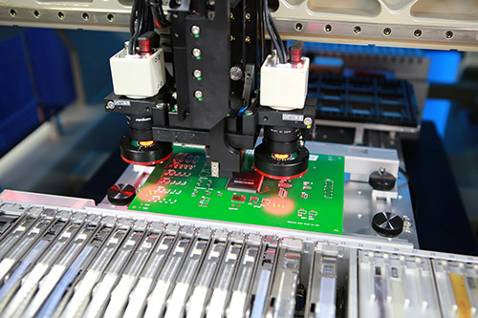
\includegraphics[width=0.8\textwidth]{images/pickandplace.png}
		\caption{Pick-and-Place machine \cite{pickandplace}}
		\label{fig:pick_and_place}
	\end{figure}
\end{minipage}%
\hfill
\begin{minipage}[h]{0.48\textwidth}
	\begin{figure}[H]
		\centering
		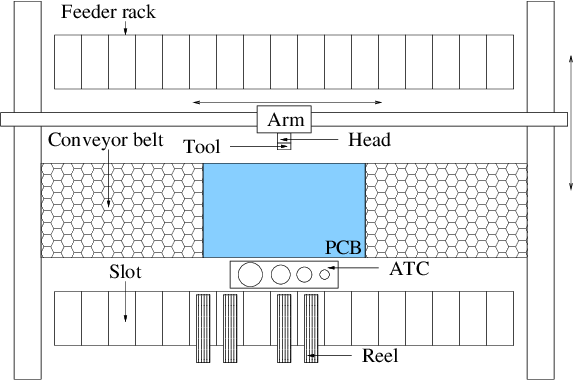
\includegraphics[width=0.8\textwidth]{images/pickandplace-diagram.png}
		\caption{Pick-and-Place machine diagram \cite{pickandplace2}}
		\label{fig:pick_and_place_diagram}
	\end{figure}
\end{minipage}

\subsection{Motivation and relevant works}
The article <<Hand-drawn electronic component recognition using deep learning algorithm>> (Wang et al.) \cite{HandDrawnRecognition} describes a similar project. The authors use a convolutional neural network (CNN) to recognize hand-drawn electronic components.

Another research, <<Integrated Circuit Packaging Recognition with Tilt Auto Adjustment using Deep Learning Approach>> (Loh et al.) \cite{ComponentsDetection}, uses YOLOv5 to detect and classify IC packages. The authors focus on IC detection on the PCB, i.e. after installation. It operates on images of the PCB, not individual IC packages.

The research <<Text Recognition in PCBs: an object character recognition algorithm>> (Nájera et al.) \cite{pickandplace} describes approaches currently used in the industry to recognize objects on PCBs. The authors use a computer vision setup on the Pick-and-Place machine head to recognize text on the PCB.

\subsection{Contribution and scope}
Mentioned researches are similar to the proposed one, but they are not directly applicable. The proposed project is focused on recognizing individual IC packages before soldering, potentially in real-time. It can then be expanded to recognize other components, such as resistors, capacitors, and inductors.

The ability to recognize ICs on the fly can significantly reduce the possibility of damage to the expensive Pick-and-Place machines and the PCBs, serving as an extra protection measure. The resulting model can be used in a computer vision setup on the feed line (<<Reel>> on Figure \ref{fig:pick_and_place_diagram}) of the Pick-and-Place machine, in addition to the existing sensors.

\section{Datasets}
A dataset of IC packages is collected from the supplier websites, mainly \href{https://digikey.com}{Digi-Key}, and \href{https://mouser.com}{Mouser}. The dataset contains images of IC packages in various resolutions and aspect ratios. The dataset is divided into four classes: SOP, QFP, SOIC, and DIP. Each class contains at least 175 images. Augmentation is performed during dataset loading and includes grayscale conversion, contrast/sharpness adjustments, and random flipping. The images are scaled and cropped to a fixed size of 128x128 pixels for better performance.

Figure \ref{fig:ic_packages} shows examples of IC packages from the dataset. Table \ref{tab:ic_packages} lists the packages and their corresponding labels.

\begin{minipage}[h]{0.48\textwidth}
	\centering
	\begin{table}[H]
	\centering
	\begin{tabular}{|l|c|c|}
	\hline
	\textbf{Package} & \textbf{Example} & \textbf{Label} \\ \hline
	SOP & 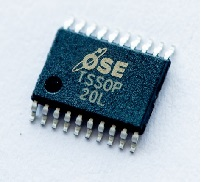
\includegraphics[width=0.2\textwidth]{images/sop.jpg} & chip-sop \\ \hline
	QFP & 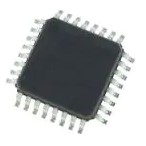
\includegraphics[width=0.2\textwidth]{images/qfp32.jpg} & chip-qfp \\ \hline
	SOIC & 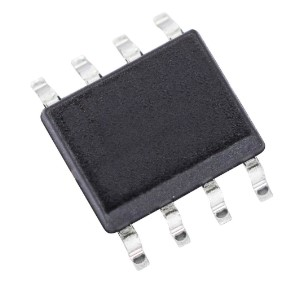
\includegraphics[width=0.2\textwidth]{images/soic8.jpg} & chip-soic \\ \hline
	DIP & 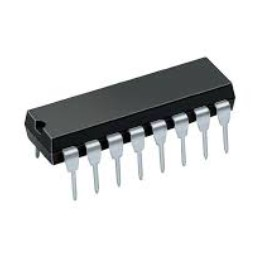
\includegraphics[width=0.2\textwidth]{images/dip16.jpg} & chip-dip \\ \hline
	\end{tabular}
	\caption{Integrated circuit packages}
	\label{tab:ic_packages}
	\end{table}
\end{minipage}%
\hfill
\begin{minipage}[h]{0.48\textwidth}
	\begin{figure}[H]
		\centering
		\subfigure[SOP]{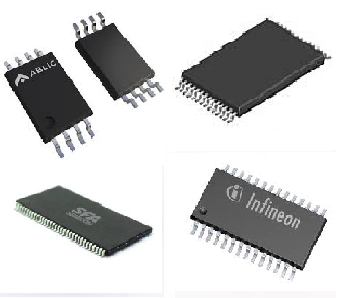
\includegraphics[width=0.4\textwidth]{images/dataset/sop.png}}
		\subfigure[QFP]{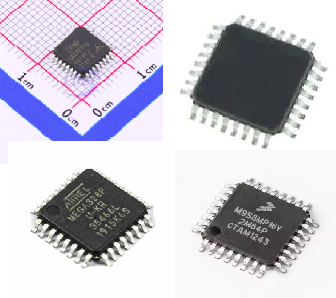
\includegraphics[width=0.4\textwidth]{images/dataset/qfp32.png}}

		\subfigure[SOIC]{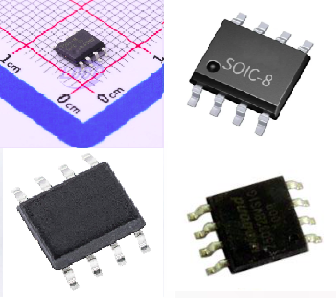
\includegraphics[width=0.4\textwidth]{images/dataset/soic8.png}}
		\subfigure[DIP]{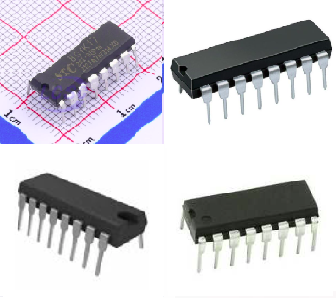
\includegraphics[width=0.4\textwidth]{images/dataset/dip16.png}}
		\caption{Integrated circuit packages from the dataset}
		\label{fig:ic_packages}
	\end{figure}
\end{minipage}

\vspace{0.5cm}
The dataset is split into training and validation sets with a 5/1 ratio. The training set contains 480 images, and the validation set contains 120 images. The dataset is balanced, with 175 images in each class. A separate test set of 20 images is used to evaluate the model's performance.

Data collection and initial classification were performed manually by the author.

\section{Methodology}
Training was performed in two stages: initial testing and hyperparameter tuning.
For the first stage, a ResNet18 CNN is used for IC package classification. Three approaches were tested: training the model from scratch, fine-tuning a pre-trained model, and using a pre-trained model as a feature extractor. The model is trained using the SGD optimizer with a batch size of 4. Cross entropy loss is used as the loss function. The model was trained for 50 epochs.

For the second stage, hyperparameter tuning was performed manually. The learning rate, weight decay, and number of epochs were varied. The best model was selected based on the validation accuracy.

Finally, confusion matrix, accuracy, precision, recall, and F1 score were calculated for the validation dataset. The model was evaluated on the test dataset to assess its generalization performance.

\section{Results}
The first stage results are shown in Table \ref{tab:stage1}. The best model was obtained by \textbf{fine-tuning a pre-trained model}. The model achieved an accuracy of 0.876 on the validation set. Severe overfitting was observed for the other two approaches, indicating issues with the dataset. Figure \ref{fig:stage1} shows one of the training runs.

\begin{table}[H]
	\centering
	\begin{tabular}{|l|c|c|c|c|}
	\hline
	\textbf{Approach} & \textbf{LR} & \textbf{Weight decay} & \textbf{Epochs} & \textbf{Validation Acc} \\ \hline
	Scratch & 0.001 & 0.01 & 50 & 0.817 \\ \hline
	Fine-tuning & 0.001 & 0.01 & 50 & 0.876 \\ \hline
	Feature extractor & 0.001 & 0.01 & 50 & 0.800 \\ \hline
	\end{tabular}
	\caption{Results for the first stage}
	\label{tab:stage1}
\end{table}

\begin{figure}[H]
	\centering
	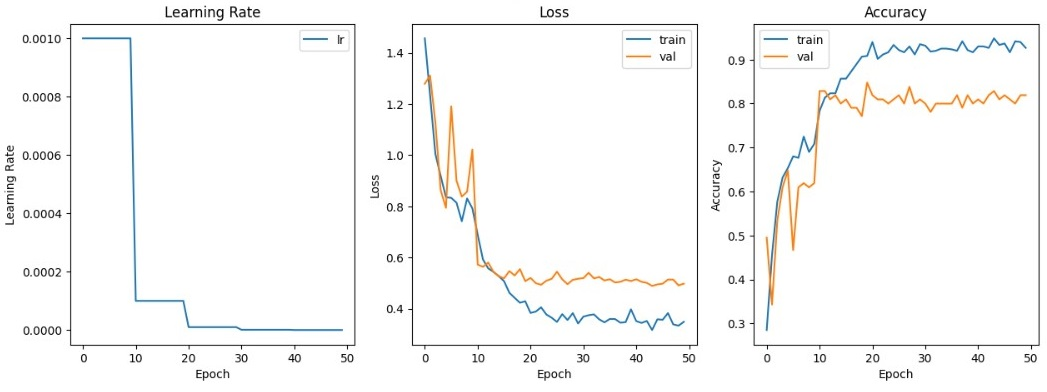
\includegraphics[width=\textwidth]{images/fromscratch.jpg}
	\caption{Training history for the From Scratch approach}
	\label{fig:stage1}
\end{figure}

It was observed that there were no improvements in the validation accuracy after 30 epochs. Therefore, the number of epochs was reduced to 30 for the second stage. 

Second stage manual optimization results are shown in Table \ref{tab:stage2}. The best model was obtained with a learning rate of 0.001, weight decay of 0.05, and 30 epochs. The model achieved an accuracy of 0.962 on the validation set. Batch size was increased to 8. Figure \ref{fig:stage2} shows the training history for the best model.

\begin{table}[H]
	\centering
	\begin{tabular}{|l|c|c|c|c|}
	\hline
	\textbf{LR} & \textbf{Weight decay} & \textbf{Epochs} & \textbf{Validation Acc} \\ \hline
	0.001 & 0.01 & 30 & 0.886 \\ \hline
	0.001 & 0.05 & 30 & 0.962 \\ \hline
	0.001 & 0.1 & 30 & 0.933 \\ \hline
	\end{tabular}
	\caption{Results for the second stage}
	\label{tab:stage2}
\end{table}

\begin{figure}[H]
	\centering
	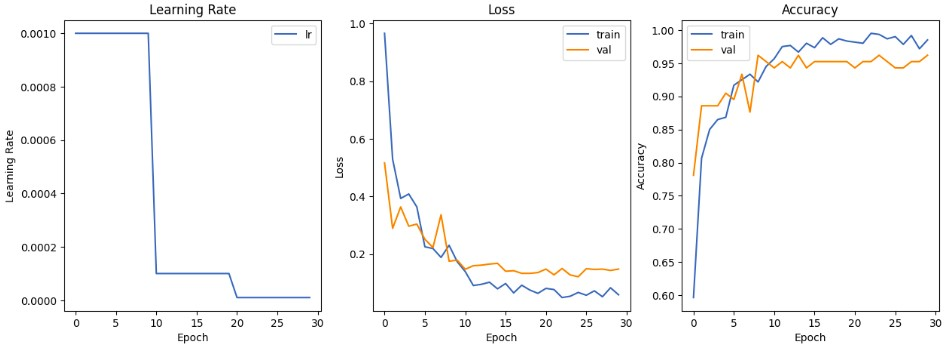
\includegraphics[width=\textwidth]{images/stage2.jpg}
	\caption{Training history for the best model, fine-tuned/pre-trained}
	\label{fig:stage2}
\end{figure}

The confusion matrix for the best model is shown in Table \ref{fig:confusion_matrix}. Table \ref{tab:metrics} shows the evaluation metrics for the best model on the validation set.

\begin{minipage}[h]{0.48\textwidth}
\begin{figure}[H]
	\centering
	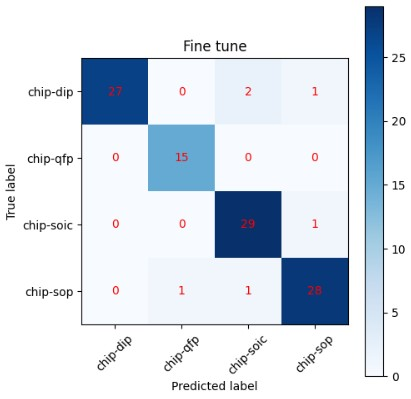
\includegraphics[width=0.8\textwidth]{images/confusion-matrix.jpg}
	\caption{Confusion matrix for the best model}
	\label{fig:confusion_matrix}
\end{figure}
\end{minipage}%
\hfill
\begin{minipage}[h]{0.48\textwidth}
\begin{table}[H]
	\centering
	\begin{tabular}{|l|c|c|c|}
	\hline
	\textbf{Class} & \textbf{Recall} & \textbf{Precision} & \textbf{F1 Score} \\ \hline
	chip-dip & 0.900 & 1.000 & 0.947 \\ \hline
	chip-qfp & 1.000 & 0.938 & 0.968 \\ \hline
	chip-soic & 0.967 & 0.906 & 0.935 \\ \hline
	chip-sop & 0.933 & 0.933 & 0.933 \\ \hline
	\textbf{Accuracy} & \multicolumn{3}{c|}{0.962} \\ \hline
	\end{tabular}
	\caption{Evaluation metrics for the best model}
	\label{tab:metrics}
\end{table}
\end{minipage}

\vspace{0.5cm}
After evaluating the model on the validation set, the model was tested on the test set. The model achieved an accuracy of 0.950 on the test set, indicating good generalization performance. Figure \ref{fig:test} shows the test results. Only one IC package was misclassified, marked in red.

\begin{figure}[H]
	\centering
	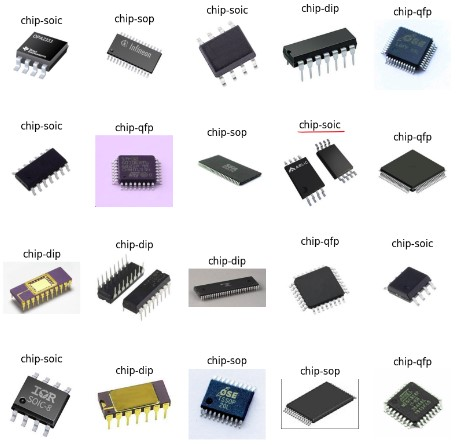
\includegraphics[width=0.8\textwidth]{images/test.jpg}
	\caption{Test results for the best model}
	\label{fig:test}
\end{figure}

\subsection{Discussion}
During training, multiple issues were observed:
\begin{itemize}
	\item The dataset was too small, leading to overfitting.
	\item Dataset collection from supplier websites has limitations, such as fixed resolutions and rotation angles.
	\item Suppliers tend to re-use images for different packages, leading to incorrect labels. This also reduces the diversity of the dataset.
	\item Some IC packages, such as SOIC-8 and SOP-8, are visually similar, leading to misclassification. It is challenging to distinguish between them even for an experienced engineer.
	\item Finally, the model was not tested on real-world data, which have different lighting conditions, angles, and backgrounds.
\end{itemize}

Considering the limitations, the model achieved good performance on the test set. The model can be further improved by collecting more data, using more advanced CNN architectures, and fine-tuning the model on real-world data.

A possible solution to the dataset limitations is to collect images of IC packages on the Pick-and-Place machine itself. This can be done by setting up a camera on the feed line of the machine and capturing images of IC packages as they pass by. The model can then be re-trained on this data to improve its performance in real-world conditions.

\section{Conclusion}
The approach to recognize integrated circuit packages using deep learning was presented. The results have shown that ResNet is a suitable architecture for IC package recognition. The best model achieved an accuracy of 0.950 on the test set, indicating good generalization performance. The model can be further improved by using a better dataset and fine-tuning the model on real-world data.

Future work includes evaluating the model in real-world conditions, and measuring the model's performance on other components, such as resistors, capacitors, and inductors. Response time will also be evaluated to determine if the model can be used in real-time applications.

The code for this project is available on GitHub: \url{https://github.com/thepetrovich/ntu-dl-term-project}.

\section*{Acknowledgments}
The author would like to thank the National Taiwan University for providing the opportunity to work on this project. The author would also like to thank Professor Rih-Teng Wu for his guidance and support throughout the project.

\bibliographystyle{unsrt}
\bibliography{references}

% \newpage
\end{document}

